% Interim report reorganized to match PolyU COMP4913 Capstone Project Handbook (2025-26).
% Source: CP Handbook_2025-26_250829.pdf
% Compile with PDFLaTeX.

\documentclass[12pt,a4paper,oneside]{report}

% --- Handbook-required layout ---
\usepackage[a4paper,left=25mm,right=20mm,top=20mm,bottom=20mm]{geometry}
\usepackage[onehalfspacing]{setspace} % at least 1.5 spacing
\usepackage{times} % Times-like font (handbook allows Times New Roman / Arial)

% --- Common report utilities ---
\usepackage{graphicx}
\usepackage{caption}
\usepackage[hyphens]{url}
\usepackage{natbib}
\usepackage{booktabs}
\usepackage{amsmath}
\usepackage[hidelinks]{hyperref} % clickable TOC/refs; keep links visually clean
\usepackage{tikz}
\usetikzlibrary{arrows.meta,positioning,shapes.geometric}

\urlstyle{rm}
\setcounter{tocdepth}{2}
\setcounter{secnumdepth}{2}

% Page numbering: top-right; title page counted but not numbered.
\usepackage{fancyhdr}
\pagestyle{fancy}
\fancyhf{}
\fancyhead[R]{\thepage}
\renewcommand{\headrulewidth}{0pt}

% --- Fill these fields (cover page only; body should not repeat personal details) ---
\newcommand{\ProjectTitle}{From Classic Strategies to Time-Series Transformers: A Quantitative Trading System (Interim Milestone)}
\newcommand{\StudentName}{Liu Chen}
\newcommand{\StudentID}{22100974D}
\newcommand{\ProgrammeStream}{BSc (HONS) Computer Science}
\newcommand{\SupervisorName}{Prof.\ Henry C.\ B.\ Chan}
\newcommand{\SubmissionDate}{31 December 2025}
% Optional (leave blank if not applicable)
\newcommand{\CoExaminer}{MIAO Hao}
\newcommand{\SecondAssessor}{LIU Yang Veronica}

\begin{document}

% -------------------- Cover page (handbook sample style) --------------------
\pagenumbering{arabic}
\thispagestyle{empty} % counted but no visible number
\setlength{\fboxsep}{14pt}
\noindent\fbox{%
\begin{minipage}[t][\dimexpr\textheight-2\fboxsep-2\fboxrule\relax]{\dimexpr\textwidth-2\fboxsep-2\fboxrule\relax}
\vspace*{6pt}
\begin{center}
{\Large\bfseries The Hong Kong Polytechnic University\\ Department of Computing}\\[34pt]

{\Large\underline{COMP4913 Capstone Project}}\\[6pt]
{\Large Report (Interim)}\\[70pt]

{\LARGE\bfseries \ProjectTitle}\\[70pt]
\end{center}

\vfill
{\Large
\noindent\begin{tabular}{@{}p{0.42\linewidth}p{0.55\linewidth}@{}}
\textbf{Student Name:} & \StudentName\\[6pt]
\textbf{Student ID No.:} & \StudentID\\[6pt]
\textbf{Programme-Stream Code:} & \ProgrammeStream\\[6pt]
\textbf{Supervisor:} & \SupervisorName\\[6pt]
\textbf{Co-Examiner:} & \CoExaminer\\[6pt]
\textbf{2\textsuperscript{nd} Assessor:} & \SecondAssessor\\[6pt]
\textbf{Submission Date:} & \SubmissionDate\\
\end{tabular}}

\vspace*{10pt}
\vspace*{6pt}
\end{minipage}%
}

\clearpage

% -------------------- Abstract --------------------
\chapter*{Abstract}
\addcontentsline{toc}{chapter}{Abstract}
This interim report documents my first end-to-end milestone of a quantitative algorithmic trading system prototype using 2800.HK daily OHLCV data. I begin with classic, interpretable strategies to validate the research loop and set a transparent baseline. I then implement a consistent ML/DL pipeline: feature engineering, volatility-adaptive 3-class labeling, fixed-window walk-forward cross-validation, and a cost-aware backtest that converts out-of-sample class probabilities into trades. Under the same protocol, I compare an LSTM baseline, a Transformer encoder baseline, and an Informer-style time-series Transformer, and I show that realized P\&L is often dominated by the probability-to-trade translation layer (thresholds, holding constraints, and costs). I further report an Informer-OPT result obtained via feature expansion, longer context, and a trading-rule parameter sweep. Finally, I integrate a news-based stage (GDELT + FinBERT) as an external signal pipeline; this stage is currently a systems milestone rather than a performance conclusion due to limited news coverage and short out-of-sample overlap.

\clearpage

% -------------------- TOC / Lists --------------------
\tableofcontents
\clearpage
\listoftables
\clearpage
\listoffigures
\clearpage

% -------------------- Main body --------------------
\chapter{Introduction}
\section{Motivation}
Financial markets are noisy and shaped by many interacting factors. While the Efficient Market Hypothesis suggests persistent alpha is difficult \citep{fama1970}, practical research can still explore short-horizon signals, provided the evaluation is time-respecting and reproducible.

\section{Midterm objective and scope}
My midterm objective is to build a complete trading research pipeline that is (i) time-respecting (no look-ahead leakage), (ii) reproducible, and (iii) able to generate standardized artifacts (metrics, plots, logs) for iterative experiments. This report presents a progressive path: classic strategies $\rightarrow$ LSTM $\rightarrow$ Transformer $\rightarrow$ Informer-style $\rightarrow$ Informer-OPT $\rightarrow$ news integration (FinBERT).

\section{Project objectives and research questions}
The interim report is expected to be comprehensive and self-contained. Therefore, I make my objectives explicit:
\begin{itemize}
  \item \textbf{O1 (Engineering):} build a reproducible pipeline that transforms raw market data into model-ready datasets, produces standardized outputs, and enables rapid iteration.
  \item \textbf{O2 (Methodology):} design a time-respecting evaluation protocol (walk-forward CV + cost-aware backtest) to avoid look-ahead bias and unrealistic assumptions.
  \item \textbf{O3 (Baselines):} establish transparent baselines (classic strategies) and progressively stronger ML/DL baselines for fair comparison.
  \item \textbf{O4 (External signals):} integrate news as an external signal source, and diagnose data alignment/coverage limitations.
\end{itemize}
This leads to the following research questions for Semester~2:
\begin{itemize}
  \item \textbf{RQ1:} Under a fixed evaluation protocol, do newer time-series Transformer architectures improve risk-adjusted performance (Sharpe, drawdown) relative to earlier baselines?
  \item \textbf{RQ2:} How sensitive is realized P\&L to the probability-to-trade translation layer (thresholds, holding constraints, costs), and how can I reduce overfitting risk in this layer \citep{bailey2014,lopezdeprado2018,white2000}?
  \item \textbf{RQ3:} Can external news signals improve predictive coverage and trading performance once sufficient news-price overlap is achieved \citep{araci2019finbert,tetlock2007}?
\end{itemize}

\chapter{Related Work and Literature Review}
\section{Algorithmic trading baselines and evaluation pitfalls}
Classic strategies (trend following, mean reversion, momentum) provide interpretable baselines and help validate backtest correctness \citep{chan2013}. However, empirical backtesting is vulnerable to data snooping and overfitting when many strategies/parameters are tested \citep{white2000,bailey2014}. For financial ML, careful validation design is essential because naive cross-validation can leak information in time series \citep{bergmeir2018}.

\section{Machine learning for financial prediction}
Sequence models such as LSTM are widely used for temporal classification and forecasting \citep{lstm1997}. In practice, performance depends not only on the model but also on labeling choices, class imbalance, probability calibration, and the trading layer that converts predictions into positions \citep{lopezdeprado2018}.

\section{Transformers for time series}
Transformers introduced self-attention as a powerful alternative to recurrence \citep{vaswani2017}. Informer improved efficiency for long sequences using ProbSparse attention and distilling \citep{informer2021}. More recent work proposes architectures specialized for time series, such as Autoformer and FEDformer, which address seasonality/trend decomposition and frequency-domain patterns \citep{autoformer2021,fedformer2022}. PatchTST (ICLR~2023) argues that patching along time and channel-independent modeling can be strong baselines, especially for multivariate series \citep{patchtst2023}. iTransformer (ICLR~2024) proposes attention over variables rather than time steps to better capture inter-variable relationships \citep{itransformer2024}.

\section{News and text-based signals}
Financial text can contain information about sentiment, uncertainty, and macro events; prior work finds that news tone can relate to market movements \citep{tetlock2007}. FinBERT adapts pretrained language models to the financial domain for sentiment analysis and related tasks \citep{araci2019finbert}. In this project, I treat news as an external signal and focus first on building a reliable alignment and evaluation pipeline before drawing performance conclusions.

\chapter{Problem Definition and Data}
\section{Instrument and data source}
\textbf{Instrument:} 2800.HK (Tracker Fund of Hong Kong), chosen for liquidity and relevance as a Hang Seng Index proxy.\\
\textbf{Data source:} Daily OHLCV from \texttt{yfinance} with auto-adjusted prices.

\section{Time span and evaluation window}
Most early experiments use three years of daily bars (period=3y, interval=1d), yielding 733 observations. When optimizing Informer with longer context windows, I expanded the history request to period=10y to preserve enough out-of-sample folds. For ML/DL models, headline metrics are reported on the final 252 out-of-sample trading days produced by walk-forward CV for that run.

\section{Prediction target}
I predict next-day close-to-close log return:
\[
r_{t+1}=\log\left(\frac{C_{t+1}}{C_t}\right).
\]

\chapter{Methodology: A Reproducible, Time-Respecting Pipeline}
\section{System framework (end-to-end workflow)}
Figure~\ref{fig:framework} summarizes the end-to-end workflow implemented in this project. The key design choice is that every model (classic or ML/DL) is evaluated under consistent assumptions: no look-ahead, explicit transaction costs, and standardized artifacts saved under \texttt{outputs/}.

\begin{center}
\captionof{figure}[System framework]{System framework of the project: data ingestion, feature engineering, labeling, walk-forward evaluation, and cost-aware backtesting.}
\label{fig:framework}
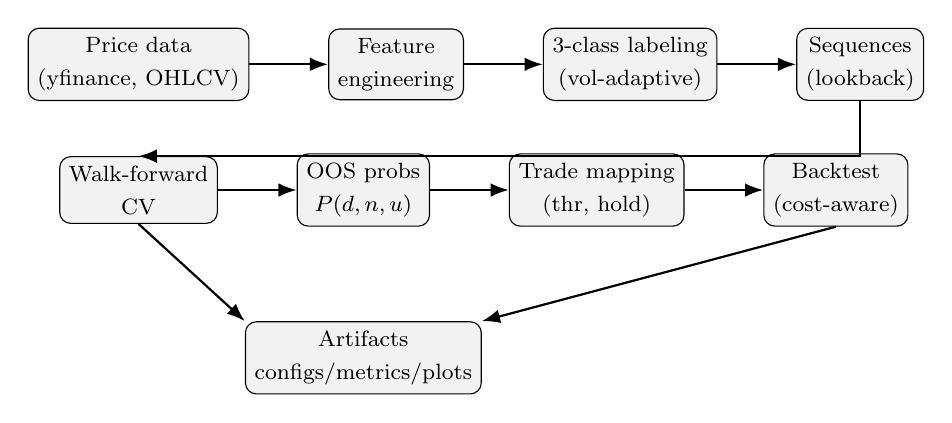
\begin{tikzpicture}[
  node distance=7mm and 10mm,
  box/.style={draw, rounded corners, align=center, minimum height=7mm, font=\footnotesize, fill=gray!10},
  arr/.style={-Latex, thick}
]
\node[box] (data) {Price data\\(yfinance, OHLCV)};
\node[box, right=of data] (feat) {Feature\\engineering};
\node[box, right=of feat] (label) {3-class labeling\\(vol-adaptive)};
\node[box, right=of label] (seq) {Sequences\\(lookback)};

\node[box, below=of data] (cv) {Walk-forward\\CV};
\node[box, right=of cv] (pred) {OOS probs\\$P(d,n,u)$};
\node[box, right=of pred] (trade) {Trade mapping\\(thr, hold)};
\node[box, right=of trade] (bt) {Backtest\\(cost-aware)};

\node[box, below=12mm of pred] (art) {Artifacts\\configs/metrics/plots};

\draw[arr] (data) -- (feat);
\draw[arr] (feat) -- (label);
\draw[arr] (label) -- (seq);

% bridge from top row to bottom row
\draw[arr] (seq.south) |- (cv.north);

\draw[arr] (cv) -- (pred);
\draw[arr] (pred) -- (trade);
\draw[arr] (trade) -- (bt);

\draw[arr] (cv.south) -- (art.north west);
\draw[arr] (bt.south) -- (art.north east);
\end{tikzpicture}
\end{center}

\section{Feature engineering}
I begin with 16 interpretable technical features: SMA(5/10/20/50), rolling variance of log returns (5/10/20), RSI(14), MACD (line/signal/histogram), and Bollinger band features. For Informer-OPT, I expand the feature set with multi-horizon returns/volatilities, ATR-based volatility, and volume-derived signals.

\section{Volatility-adaptive 3-class labeling}
I use a dynamic threshold tied to recent volatility to reduce regime sensitivity. Let $\sigma^{(20)}_t$ be the rolling standard deviation of 1-day log returns over a 20-day window, shifted by one day to avoid leakage. The threshold is:
\[
\tau_t=\max(\text{min\_vol},\,k\cdot\sigma_{t}^{(20)}),\quad k=0.8,\ \text{min\_vol}=10^{-4}.
\]
Labels: Up if $r_{t+1}\ge \tau_t$, Down if $r_{t+1}\le -\tau_t$, else Neutral.

\section{Walk-forward cross-validation}
I use fixed-window walk-forward splits with train/validation/test windows and step size chosen to avoid lookahead leakage. Standardization is fit on each training split only and applied to validation/test.

\section{From probabilities to trades (cost-aware backtest)}
For each out-of-sample day, the model outputs probabilities $(P(\text{Down}),P(\text{Neutral}),P(\text{Up}))$. I apply a confidence threshold: if $\max P < \text{thr}$, I force Neutral (no trade). Otherwise, I map to a discrete position (long/short) and enforce a minimum holding period to reduce flip-flopping. Transaction cost is charged on absolute position changes at 2 bps. This ``translation layer'' is evaluated explicitly because it often dominates realized P\&L \citep{bailey2014,lopezdeprado2018}.

\section{Preliminary metrics}
In addition to total return, I report risk and behavior metrics that help diagnose why a strategy may underperform Buy\&Hold:
\begin{itemize}
  \item \textbf{Sharpe ratio} (risk-adjusted return)
  \item \textbf{Maximum drawdown} (tail risk and path dependency)
  \item \textbf{Coverage} (fraction of days holding a non-zero position)
  \item \textbf{Turnover / trades} (trading intensity and sensitivity to transaction costs)
\end{itemize}

\chapter{Classic Strategy Baselines (Pre-ML)}
\section{Why classic baselines first}
Before ML/DL, I implemented classic, interpretable strategies to validate the data/backtest loop and build intuition for 2800.HK \citep{chan2013}. These baselines are not optimized; they provide a transparent benchmark.

\section{Representative results (3-year sample)}
Table~\ref{tab:classic_bt} summarizes representative classic strategies (3-year sample, costs included).

\begin{center}
\small
\captionof{table}[Classic strategy baselines (3-year sample)]{Classic strategy baselines on 2800.HK (full 3-year sample; 2 bps transaction cost). Some strategies show strong risk-adjusted metrics but trail Buy\&Hold in total return due to low exposure and trading frictions.}
\label{tab:classic_bt}
\begin{tabular}{lrrrr}
\toprule
Strategy & Total ret. & Sharpe & Max DD & Coverage \\
\midrule
RSI & 0.1325 & 1.2977 & -0.0029 & 0.0109 \\
Bollinger (MR) & 0.0735 & 0.4944 & -0.0998 & 0.0464 \\
Dual MA (10/50) & 0.1075 & 0.2864 & -0.2010 & 0.4911 \\
Donchian (20/10) & -0.0275 & 0.0047 & -0.2164 & 0.3438 \\
\midrule
Buy\&Hold (same 3y) & 0.4436 & -- & -- & 1.0000 \\
\bottomrule
\end{tabular}
\end{center}

\begin{center}
\includegraphics[width=0.85\textwidth]{classic_rsi_backtest_20251229_220548.png}
\captionof{figure}[RSI baseline]{Classic baseline example: RSI mean-reversion (equity curve and position).}
\label{fig:classic_rsi}
\end{center}

\begin{center}
\includegraphics[width=0.85\textwidth]{classic_dualma10_50_backtest_20251229_220548.png}
\captionof{figure}[Dual MA baseline]{Classic baseline example: Dual moving-average trend (equity curve and position).}
\label{fig:classic_dualma}
\end{center}

\chapter{ML/DL Experiments Under a Consistent Protocol}
\section{LSTM baseline (first reproducible ML run)}
I train a PyTorch LSTM multi-class classifier with lookback=30 and 16 features. The run produces standardized artifacts: configuration snapshot, walk-forward CV metrics, per-day probabilities, and a cost-aware backtest on the last 252 out-of-sample trading days.

\begin{center}
\small
\captionof{table}[LSTM backtest summary]{Backtest summary for the LSTM baseline (last \textasciitilde 1 year out-of-sample; costs included).}
\label{tab:lstm_bt}
\begin{tabular}{lrr}
\toprule
Metric & LSTM Strategy & Buy\&Hold \\
\midrule
Days & 252 & 252 \\
Total return & -0.0623 & 0.2230 \\
Annualized return & -0.0623 & 0.2230 \\
Annualized volatility & 0.1033 & -- \\
Sharpe ratio & -0.5711 & -- \\
Max drawdown & -0.1344 & -- \\
Position coverage & 0.2540 & 1.0000 \\
\bottomrule
\end{tabular}
\end{center}

\begin{center}
\includegraphics[width=0.90\textwidth]{lstm2_backtest_20251229_183712.png}
\captionof{figure}[LSTM backtest]{LSTM backtest visualization (equity, position, probabilities).}
\label{fig:lstm_bt}
\end{center}

\section{Transformer encoder baseline (GPU run)}
I implement a Transformer encoder classifier and evaluate it under the same protocol \citep{vaswani2017}. This increases model capacity and enables stronger sequence modeling without recurrence.

\begin{center}
\small
\captionof{table}[Transformer backtest summary]{Backtest summary for the Transformer baseline (last \textasciitilde 1 year out-of-sample; costs included).}
\label{tab:tx_bt}
\begin{tabular}{lrr}
\toprule
Metric & Transformer Strategy & Buy\&Hold \\
\midrule
Days & 252 & 252 \\
Total return & 0.0094 & 0.2230 \\
Annualized return & 0.0094 & 0.2230 \\
Annualized volatility & 0.2173 & -- \\
Sharpe ratio & 0.1482 & -- \\
Max drawdown & -0.1732 & -- \\
Position coverage & 0.6230 & 1.0000 \\
\bottomrule
\end{tabular}
\end{center}

\begin{center}
\includegraphics[width=0.90\textwidth]{transformer_backtest_20251229_125307.png}
\captionof{figure}[Transformer backtest]{Transformer backtest visualization (equity, position, probabilities).}
\label{fig:tx_bt}
\end{center}

\section{Informer-style time-series Transformer}
I implement an Informer-inspired encoder classifier with ProbSparse attention and optional distilling to explore efficient long-sequence mechanisms \citep{informer2021}. Early trials highlight that the trading-rule parameters (confidence threshold and holding period) can suppress trading or concentrate exposure unintentionally; therefore, I treat the trading layer as part of the evaluated system \citep{bailey2014,lopezdeprado2018}.

\begin{center}
\small
\captionof{table}[Informer-style backtest summary]{Backtest summary for the Informer-style baseline (last \textasciitilde 1 year out-of-sample; costs included).}
\label{tab:inf_bt}
\begin{tabular}{lrr}
\toprule
Metric & Informer-style & Buy\&Hold \\
\midrule
Days & 252 & 252 \\
Total return & -0.0102 & 0.2230 \\
Sharpe ratio & -0.0119 & -- \\
Max drawdown & -0.1528 & -- \\
Position coverage & 0.4206 & 1.0000 \\
Turnover (avg $|\Delta pos|$) & 0.0595 & -- \\
Trades (pos changes) & 14 & -- \\
\bottomrule
\end{tabular}
\end{center}

\begin{center}
\includegraphics[width=0.90\textwidth]{informer_backtest_20251229_144632.png}
\captionof{figure}[Informer-style backtest]{Informer-style backtest visualization (equity, position, probabilities).}
\label{fig:inf_bt}
\end{center}

\section{Informer-OPT: feature expansion + longer context + trading-rule sweep}
I then perform a structured optimization: expand features, increase temporal context, switch to a full 3-class loss for better calibration, and sweep the trading-rule parameters without retraining the model. The best configuration from the sweep nearly matches Buy\&Hold over the same window with lower drawdown and modest turnover.

\begin{center}
\small
\captionof{table}[Informer-OPT best result]{Informer-OPT best result from trading-rule sweep.}
\label{tab:inf_opt}
\begin{tabular}{lrr}
\toprule
Metric & Informer-OPT (best) & Buy\&Hold \\
\midrule
Days & 252 & 252 \\
Total return & 0.3675 & 0.3692 \\
Excess return & -0.0017 & -- \\
Annualized volatility & 0.1677 & -- \\
Sharpe ratio & 1.9501 & -- \\
Max drawdown & -0.0751 & -- \\
Position coverage & 0.6905 & 1.0000 \\
Trades (pos changes) & 7 & -- \\
Trading rule & thr=0.36, hold$\ge$5, long-only & -- \\
\bottomrule
\end{tabular}
\end{center}

\begin{center}
\includegraphics[width=0.90\textwidth]{informer_opt_backtest_20251229_152746.png}
\captionof{figure}[Informer-OPT backtest]{Informer-OPT backtest visualization (equity, position, probabilities).}
\label{fig:inf_opt}
\end{center}

\chapter{News as an External Signal (FinBERT Integration)}
\section{Motivation: why news, and why it relates to 2800.HK}
Price-only signals may miss external drivers. Because 2800.HK tracks a broad HK equity index, macro and market news can influence next-day sentiment and flows. In this stage, my goal is to build a scalable news-to-trade workflow that can be evaluated once coverage is sufficient.

\section{Data acquisition (GDELT) and preprocessing}
I use the GDELT 2.1 Document API to fetch news, map it to HK tickers via alias queries, and aggregate text by (date,ticker). The processed dataset is stored as \texttt{data/news/news.csv} with schema \texttt{date,ticker,text}.

\section{Pretrained model and fine-tuning objective}
I start from FinBERT (\texttt{ProsusAI/finbert}) \citep{araci2019finbert} and attempt to fine-tune it to predict next-day direction labels (Down/Neutral/Up), treating the output as a news-sentiment/news-signal classifier. I then convert probabilities to positions and backtest an equal-weight HK portfolio.

\section{Interim status}
The pipeline runs end-to-end and produces alignment diagnostics, but the out-of-sample window is currently very short due to limited overlap between news and price dates. Therefore, this stage is reported as a systems milestone rather than a performance conclusion.

\begin{center}
\includegraphics[width=0.90\textwidth]{finbert_portfolio_backtest_20251230_143439.png}
\captionof{figure}[FinBERT-news backtest]{FinBERT-news portfolio backtest visualization (short window due to limited news coverage).}
\label{fig:finbert_bt}
\end{center}

\chapter{Preliminary Results and Discussion}
\section{What the baselines tell me about 2800.HK}
Classic strategies provide an interpretability-first reference. Table~\ref{tab:classic_bt} and Figures~\ref{fig:classic_rsi}--\ref{fig:classic_dualma} show that:
\begin{itemize}
  \item Mean-reversion rules (e.g., RSI) can achieve attractive Sharpe but may have \textbf{very low coverage}, which reduces total return in a rising market regime.
  \item Trend rules (e.g., Dual MA) increase exposure but can suffer from whipsaws and larger drawdowns when the market is choppy.
\end{itemize}
This baseline phase also validated that the backtest implementation behaves as expected under simple, interpretable signals \citep{chan2013}.

\section{ML/DL results: performance vs exposure trade-off}
Across ML/DL baselines, I observe a consistent trade-off between \textbf{coverage} (how often I hold risk) and \textbf{net performance after costs}. For example:
\begin{itemize}
  \item The LSTM baseline (Table~\ref{tab:lstm_bt}, Figure~\ref{fig:lstm_bt}) has low coverage and underperforms Buy\&Hold on the last 252 out-of-sample days.
  \item The Transformer baseline (Table~\ref{tab:tx_bt}, Figure~\ref{fig:tx_bt}) increases coverage substantially but only slightly improves total return, still trailing Buy\&Hold.
\end{itemize}
In other words, higher model capacity does not automatically translate to better trading performance; the signal must be both \emph{predictive} and \emph{actionable under costs}.

\section{The translation layer is a first-order effect (and a risk)}
The Informer experiments highlight a key system-level insight: probability-to-trade mapping can dominate realized P\&L. The Informer-style baseline underperforms (Table~\ref{tab:inf_bt}, Figure~\ref{fig:inf_bt}), but Informer-OPT (Table~\ref{tab:inf_opt}, Figure~\ref{fig:inf_opt}) approaches Buy\&Hold with fewer trades and lower drawdown after tuning calibration and trading rules.

This is encouraging as an engineering milestone, but it also raises a methodological risk: \textbf{overfitting the trading rule} when many thresholds/holding periods are tried on the same out-of-sample series \citep{white2000,bailey2014}. In Semester~2, I will treat the trading layer as part of the model selection process and constrain parameter searches to reduce data snooping.

\section{News stage: why the result is not yet conclusive}
The news pipeline (GDELT + FinBERT) is implemented end-to-end and produces a portfolio backtest plot (Figure~\ref{fig:finbert_bt}). However, the current out-of-sample overlap is short due to limited news coverage and alignment. Therefore:
\begin{itemize}
  \item I treat this stage as a \textbf{systems milestone} rather than a performance result.
  \item The immediate next step is to increase news coverage and ensure a sufficiently long test period before evaluating whether news improves predictions \citep{leetaru2013gdelt,araci2019finbert,tetlock2007}.
\end{itemize}

\section{Threats to validity and interim limitations}
The interim results should be interpreted with the following limitations:
\begin{itemize}
  \item \textbf{Single-instrument focus:} most price-only experiments are on 2800.HK, which limits generality. Multi-asset evaluation is planned.
  \item \textbf{Transaction costs and slippage:} I include 2 bps costs, but real execution may be worse; robustness checks are needed.
  \item \textbf{Multiple testing risk:} sweeping trading parameters can inflate apparent performance if not handled carefully \citep{white2000,bailey2014}.
  \item \textbf{News coverage:} current text-based evaluation is constrained by missing/imbalanced news days.
\end{itemize}

\chapter{Progress Summary and Lessons Learned}
\section{What I have achieved so far}
By midterm, I have achieved the following deliverables:
\begin{itemize}
  \item A reproducible pipeline that produces standardized artifacts in \texttt{outputs/} (configs, CV metrics, per-day predictions, backtest statistics, and plots).
  \item Classic strategy baselines that validate the backtest mechanics and provide transparent benchmarks.
  \item ML/DL baselines (LSTM, Transformer, Informer-style) evaluated under a consistent time-respecting protocol.
  \item An explicit optimization step (Informer-OPT) that demonstrates the importance and risk of the probability-to-trade translation layer.
  \item A first integrated news stage (GDELT + FinBERT) with data alignment diagnostics, setting up the next research phase.
\end{itemize}

\section{Key lessons}
Time-respecting evaluation is non-negotiable \citep{bergmeir2018}. In addition, backtests can be overfit at the trading-rule layer even without retraining the model \citep{bailey2014,lopezdeprado2018}. Finally, data coverage and alignment constrain what can be concluded from news-based modeling.

\chapter{Work Plan (Next Stage)}
To progress from a systems milestone to a defensible research result, my next steps are:
\begin{itemize}
  \item \textbf{Stronger time-series baselines (PatchTST / iTransformer).} Implement and evaluate newer architectures under the same walk-forward protocol to test whether the architecture upgrade improves Sharpe and drawdown \citep{patchtst2023,itransformer2024}.
  \item \textbf{News coverage expansion and alignment.} Increase GDELT coverage by time-sliced collection and deduplication, and ensure the out-of-sample overlap exceeds a minimum number of trading days before drawing conclusions \citep{leetaru2013gdelt,araci2019finbert}.
  \item \textbf{Robust evaluation against overfitting.} Reduce the risk of overfitting at the trading-rule layer by limiting parameter sweeps, using out-of-sample constraints, and applying statistical checks (e.g., reality check / multiple testing awareness) \citep{white2000,bailey2014}.
  \item \textbf{Multi-asset and portfolio view.} Expand beyond single-instrument backtests to a small HK universe and evaluate portfolio-level decisions under realistic costs.
  \item \textbf{Ablation and interpretability.} Perform ablations on features, labeling thresholds, and calibration to understand which components drive improvements and which add noise.
\end{itemize}

\chapter{Conclusion}
This interim report documents a complete, time-respecting trading research pipeline and a sequence of progressively stronger baselines. While most price-based ML/DL runs do not beat Buy\&Hold in total return, the experiments establish a reproducible evaluation framework and reveal that the probability-to-trade translation layer is a dominant driver of realized performance. The news stage (GDELT + FinBERT) is integrated and debuggable, and the next phase is to expand coverage so that text-based signals can be evaluated fairly.

% -------------------- References (10 items, consistent with earlier report) --------------------
\bibliographystyle{plainnat}
\begin{thebibliography}{}
\bibitem[Fama 1970]{fama1970}
Fama, E. F. 1970.
Efficient capital markets: A review of theory and empirical work.
\textit{Journal of Finance} 25(2):383--417.

\bibitem[Chan 2013]{chan2013}
Chan, E. P. 2013.
\textit{Algorithmic Trading: Winning Strategies and Their Rationale}.
John Wiley \& Sons.

\bibitem[Bergmeir, Hyndman, and Koo 2018]{bergmeir2018}
Bergmeir, C.; Hyndman, R. J.; and Koo, B. 2018.
A note on the validity of cross-validation for evaluating autoregressive time series prediction.
\textit{Computational Statistics \& Data Analysis} 120:70--83.

\bibitem[Bailey et al.\ 2014]{bailey2014}
Bailey, D. H.; Borwein, J. M.; López de Prado, M.; and Zhu, Q. J. 2014.
The probability of backtest overfitting.
\textit{Journal of Computational Finance} 20(4):39--69.

\bibitem[White 2000]{white2000}
White, H. 2000.
A reality check for data snooping.
\textit{Econometrica} 68(5):1097--1126.

\bibitem[López de Prado 2018]{lopezdeprado2018}
López de Prado, M. 2018.
\textit{Advances in Financial Machine Learning}.
John Wiley \& Sons.

\bibitem[Hochreiter and Schmidhuber 1997]{lstm1997}
Hochreiter, S.; and Schmidhuber, J. 1997.
Long short-term memory.
\textit{Neural Computation} 9(8):1735--1780.

\bibitem[Vaswani et al.\ 2017]{vaswani2017}
Vaswani, A.; Shazeer, N.; Parmar, N.; Uszkoreit, J.; Jones, L.; Gomez, A. N.; Kaiser, \L.; and Polosukhin, I. 2017.
Attention is all you need.
In \textit{Advances in Neural Information Processing Systems (NeurIPS)}.

\bibitem[Zhou et al.\ 2021]{informer2021}
Zhou, H.; Zhang, S.; Peng, J.; Zhang, S.; Li, J.; Xiong, H.; and Zhang, W. 2021.
Informer: Beyond Efficient Transformer for Long Sequence Time-Series Forecasting.
In \textit{Proceedings of AAAI}.

\bibitem[Wu et al.\ 2021]{autoformer2021}
Wu, H.; Xu, J.; Wang, J.; and Long, M. 2021.
Autoformer: Decomposition transformers with auto-correlation for long-term series forecasting.
In \textit{Advances in Neural Information Processing Systems (NeurIPS)}.

\bibitem[Zhou et al.\ 2022]{fedformer2022}
Zhou, T.; Ma, Z.; Wen, Q.; Wang, X.; Sun, L.; and Jin, R. 2022.
FEDformer: Frequency enhanced decomposed transformer for long-term series forecasting.
In \textit{Proceedings of ICML}.

\bibitem[Nie et al.\ 2023]{patchtst2023}
Nie, Y.; Huan, L.; Wen, Q.; Wang, X.; and Jin, R. 2023.
A time series is worth 64 words: Long-term forecasting with transformers.
In \textit{Proceedings of ICLR}. (PatchTST)

\bibitem[Liu et al.\ 2024]{itransformer2024}
Liu, Y.; Zhang, H.; Li, J.; and others. 2024.
iTransformer: Inverted transformers are effective for time series forecasting.
In \textit{Proceedings of ICLR}.

\bibitem[Araci 2019]{araci2019finbert}
Araci, D. 2019.
FinBERT: Financial sentiment analysis with pre-trained language models.
\textit{arXiv preprint arXiv:1908.10063}.

\bibitem[Tetlock 2007]{tetlock2007}
Tetlock, P. C. 2007.
Giving content to investor sentiment: The role of media in the stock market.
\textit{The Journal of Finance} 62(3):1139--1168.

\bibitem[Leetaru and Schrodt 2013]{leetaru2013gdelt}
Leetaru, K.; and Schrodt, P. A. 2013.
GDELT: Global data on events, location, and tone.
In \textit{ISA Annual Convention (poster)}.
\end{thebibliography}

\end{document}


